\documentclass{report}
\usepackage{hyperref}
\usepackage{fontspec}
\usepackage{amsmath} 
\usepackage{graphicx}
\usepackage{nopageno}
\usepackage{courier}
\usepackage{listings}
\usepackage{parskip}
\usepackage{framed}
\usepackage{tikz}
\usetikzlibrary{arrows,positioning}
%\usepackage{ulem}
\setmonofont{Noto Mono}
%\newfontfamily{\Courier}{Nimbus Mono PS}
%\setmainfont{AR PL UKai TW}
\setmainfont{Times New Roman}
\renewcommand{\ttdefault}{pcr}
\XeTeXlinebreaklocale "zh"
\usepackage[a4paper, total={6in, 8in}]{geometry}
\pagestyle{plain}
\newcommand{\bs}{\textbackslash}

\usepackage{xcolor}
\usepackage{listings}
\lstset{escapeinside={<@}{@>}}
\definecolor{mGreen}{rgb}{0.2,0.8,0.2}
\definecolor{mGray}{rgb}{0.5,0.5,0.5}
\definecolor{mRed}{rgb}{1.0,0,0}
\definecolor{backgroundColour}{rgb}{0,0,0}
\definecolor{mWhite}{rgb}{0.9,0.9,0.9}
\lstset{basicstyle=\tt}
\lstdefinestyle{CStyle}{
    backgroundcolor=\color{backgroundColour},   
    commentstyle=\color{mGray},
    keywordstyle=\color{mGreen},
    numberstyle=\color{mGray},
    stringstyle=\color{mRed},
    basicstyle=\color{mWhite}\tt,
    breakatwhitespace=false,         
    breaklines=true,                 
    captionpos=b,                    
    keepspaces=true,                 
    numbers=left,                    
    numbersep=5pt,                  
    showspaces=false,                
    showstringspaces=false,
    showtabs=false,                  
    tabsize=2,
    language=C
}

\title{A Handout For Students in Kan Chiao}
\author{Handsome Liu}

\begin{document}
\fontsize{12pt}{16pt}\selectfont
\maketitle
\tableofcontents
\part{Introduction}
\chapter{C/C++ Programming Language}
\section{Programming Language}
\subsection{Programming Language and Natural Language}

    Different from \textbf{natural language}, the language that we using to communicate with other \textit{human beings}, \textbf{programming language} is a kind of language that we using to communicate with \textit{machines}.

    As you may expect, computers are not smart enough to comprehend C/C++ programming language directly. The language used by CPUs is called \textit{machine code}. As a result, we need a \textbf{compiler} to achieve such translation. The concept of \textbf{compile} and \textbf{interpret} will be introduced in later section.\\

    \begin{framed}
    \begin{center}
    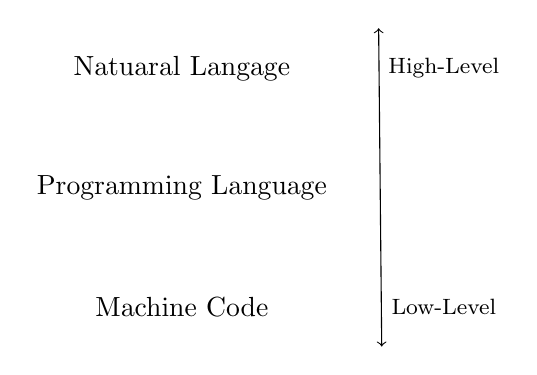
\begin{tikzpicture}[node/.style={rectangle,minimum height=10mm},node distance=5mm]
    \node(nl)[node]   {Natuaral Langage};
    \node(pl)[node,below= of nl]   {Programming Language};
    \node(mc)[node,below= of pl]   {Machine Code};
    \node(hl)[node,right=1cm of nl]   {\footnotesize High-Level};
    \node(ml)[node,below= of hl]   {};
    \node(ll)[node,below= of ml]   {\footnotesize Low-Level};
    \draw [<->] (hl.north west)--(ll.south west);
    \end{tikzpicture}
    \end{center}
    \end{framed}
    
\subsection{Source File}
    The code you wrote is called the \textbf{source code}, and the file containing your source code is called the \textbf{source file}.

\subsection{Compile and Interpret}

    To \textbf{compile} means to translate \textit{the whole source file} into another language, say, machine code.

    To \textbf{interpret} means to translate the source code \textit{line by line} and execute it immediately.

    Programming languages that needs to be compiled are called \textbf{compiled language}, while those that needs to be interpreted are called \textbf{interpreted language}.

\section{C/C++ Language}
    
    C programming language is a programming language developed by \textit{Dennis Ritchie} in 1969 ~ 1973. It is general-purpose, efficient and easy-to-read, which makes it the first choice for informatics competition.

    Based on the syntax of C, \textit{Bjarne Stroustrup} create C++ programming language to achieve \textit{OOP (object-oriented programming)}. 
    
    \subsection{Source File and Header File}

    Sometimes, it's kind of stupid to define all things in a single file. In C/C++, you can define things in some other files. The file that contains the \texttt{main()} function is called \textbf{source file}, and the files you used to define things in them are called \textbf{header files}. In this book, we will not learn how to write your own header files, but we will learn how to use others' header files.

    \subsection{Compiler for C/C++}

    C and C++ are both \textbf{compiled languages}, which means we need a compiler to compile your source code in order to execute it. The most-used one in Windows system is called \texttt{mingw}, while the most-used one in Linux system is called \texttt{gcc}.

\section{IDE (Intergrated Development Environment)}

    IDE is a kind of application that provides facilities to programmers for coding. An IDE usually consists of:
    \begin{itemize}
    \item a code editor (with syntax highlighter)
    \item automatically building tools (call the compiler to compile your source code, and execute it automatically)
    \item a debugger (tells you which line of your code disobeys the rule of syntax)
    \end{itemize}

    \subsection{Code::Blocks}

    \textit{Code::Blocks} is a free, open-source IDE that supports many programming languages. Actually, Code::Blocks itself is developed in C++.

\section{Run on Your PC}

    \subsection{IDE and Compiler Installation}
    
    Go to \url{http://www.codeblocks.org/downloads/26}.

    If you are using Windows, please choose \textit{codeblocks-xx.xxmingw-setup.exe}.

    If you are using Linux, please choose the one corresponding the operating system you use.
        
    If you are using Mac, you don't have any choice, just press the only link for Mac OS X.

    After downloading, follow the installation guide until the installation is complete.

    \subsection{Test}

    After finishing the installation, press \texttt{Ctrl+Shift+N} to open a new file. Paste the code below, and press the button with gear and green triangle to execute it.

\begin{lstlisting}[style=CStyle]
#include<stdio.h>
int main(){
    printf("Handsome Liu is so handsome!\n");
}
\end{lstlisting}

    If you've done all the steps above correctly, you should see a windows with text \texttt{ Handsome Liu is so handsome! } on it. However, if there is not, please check all the steps again.

\part{Getting Started}
\chapter{Basic Concepts}
    In this chapter, we will introduce some basic concepts you need to know.
\section{Data Type}
    As you have known, computers stores binary data. However, to we human beings, binary data is hard to manipulate or to read. Data types are some ways to interpret those binary data.
   
    \subsection{Fundamental Data Type}
    Fundamental data types, or built-in data types, are provided by the compiler, so you can simply use it without define them.

    There are 3 common fundamental data types you need to know, and will be discussed in the later chapters. They are integers (\texttt{int}), characters (\texttt{char}), and floating point numbers (\texttt{double}).

    \subsection{Derived Data Type}
    Derived data types are some data types that need to be constructed with advanced syntax. Using them, you can create new data types from fundamental data type.

    There are many derived data types in C/C++, such as array, structure, union, pointer, and enumeration. We will focus on array and pointer in later chapters.

\section{Keyword}
    Keywords, or reserved words, are some words that have fixed meaning in C/C++, and you should NOT name variables after them, just like you should not name a person "He" or "They".

    The following list are the keywords in C/C++.
\begin{lstlisting}
and              and_eq          asm
auto             bitand          bitor
bool             break           case
catch            char            class
compl            const           const_cast
continue         default         delete
do               double          dynamic_cast
else             enum            explicit
export           extern          false
float            for             friend
goto             if              inline
int              long            mutable
namespace        new             not
not_eq           operator        or
or_eq            private         protected 
public           register        reinterpret_cast
return           short           signed
sizeof           static          static_cast
struct           switch          template
this             throw           true
try              typedef         typeid
typename         union           unsigned
using            virtual         void
volatile         wchar_t         while
xor              xor_eq 
\end{lstlisting}

\section{Identifier}
    Identifier is a kind of string that can be used to name a variable. An legal identifier only contains capital English alphabets, small English alphabets, numeric characters and underscore, and begin with non-numeric characters.

    Capital English alphabets: \texttt{ABCDEFGHIJKLMNOPQRSTUVWXYZ}\\
    Small English alphabets: \texttt{abcdefghijklmnopqrstuvwxyz}\\
    Numeric characters: \texttt{0123456789}\\
    Underscore: \texttt{\_}\\

Examples:
\begin{lstlisting}
    handsomeLiu
    HandsomeLiu
    HandsomeLiu012
    handsome_liu_012
    __handsomeLiu
    ____
\end{lstlisting}
Non-examples:
\begin{lstlisting}
    <@\textcolor{red}{0}@>12handsomeLiu  (begin with numeric characters)
    handsome<@\textcolor{red}{-}@>liu    (hyphen (-))
    handsome<@\colorbox{red!20}{\color{red!20}}@>liu    (space ( ))
\end{lstlisting}

    
\section{Variable}
    Variable is a method to store data. You can use the variable as the value it stores.

    Before using a variable, you need to declare it, which means to specify its data type and name. After declared, the data type and the name of a variable cannot be changed. A variable should be named after an identifier.

\section{Statement}
    Statements are fragments of the program that are executed in sequence. In general cases, the statements will be executed line by line, from up to down. However, there are some statements allows the program execute the statements in different order, which bring us more convenience.

    \subsection{Branching Statements}
    Branching statements allows the program do different things under different condition. There are two branching statements in C/C++. They are \texttt{if-else} and \texttt{switch}.
    \subsection{Iteration Statements}
    Iteration, or loop, means to do a procedure repeatedly. To start a iteration, you can use iteration statements. These statements provide different ways to control how many times the procedure will be executed. There are three iteration statements in C/C++. They are \texttt{while}, \texttt{for}, and \texttt{do}.
    \subsection{Jump Statements}
    Jump statements cause a jump to another statement elsewhere in the code. Generally, they are used to interrupt \texttt{switch} statement and iteration staements. The jump statements are \texttt{break}, \texttt{continue} and \texttt{goto}. 

\section{Operand and Operator}
    The operand is the operated object, while the operator is the symbol specifying the type of operation.

    For example, in the operation 8+9, both 8 and 9 are operand, and + is the operator.

    There are four kinds of operators in C/C++. They are arithmetic operators, relational operators, logical operators, and bitwise operators.

    Arithmetic operators are used to perform mathematical computation, such as addition, substraction, and so on.

    Relational operators are used for comparison the values of two operands, such as equality, inequality and so on.

    Logical operators are used to manipulate some conditions, such as 'and', 'or', and 'not'.

    Bitwise operators are used to perform operations on binary numbers, which will not be discussed in this book.

\chapter{Structure of a C/C++ Program}
We will use the following program as an example.
\begin{lstlisting}[style=CStyle]
#include<stdio.h>
int main(){
    printf("Handsome Liu is so handsome!\n");
    /*This
      is
      a
      comment*/
    //This is also a comment
}
\end{lstlisting}

\section{Including the Header Files}
\begin{lstlisting}[style=CStyle]
#include<stdio.h>
\end{lstlisting}
As mentioned before, some functions are defined in other header files. \texttt{stdio.h} is a header file provided by the compiler. \texttt{stdio} stands for STanDard Input and Output. Since \texttt{printf} is defined in \texttt{stdio.h}, we need to specify that we want to use \texttt{stdio.h}. The syntax for using a header file is
\begin{center}\texttt{\#include< <header\_file> >}\end{center}
\section{The \texttt{main} Function}
\begin{lstlisting}[style=CStyle,firstnumber=2]
int main(){
\end{lstlisting}
\begin{lstlisting}[style=CStyle,firstnumber=9]
}
\end{lstlisting}
The \texttt{main} function is the starting point of every program. A program always start to execute from the \texttt{main} function.
\section{Comments}
Comments are written for human beings, not compilers. Compilers will ignore all contents inside comments.

A comment can be construct by two ways, \texttt{//} or a pair of \texttt{/*}  and \texttt{*/}.

All contents after \texttt{//} will be viewed as comments until the end of the line.\\
All contents after \texttt{/*} will be viewed as comments until \texttt{*/}.\\

\chapter{Basic Syntaxes}
In this chapter, we will learn about how to implement the concepts in chapter 2.

\section{Value and Literal}
    We have learned that there are many different type of value, such as integers, characters, and floating point numbers. A literal is a representation of the value. For example, an integer 3 and a character 3 should have different representations.
    \subsection{Integer Literal}
        To represent a decimal integer, just type it down like in mathematics. For example, \texttt{123} represents the integer one hundred and twenty-three.

    \subsection{Character Literal}
        To represent a character, enclose the character with a pair of single quotation marks. For example, \texttt{'A'} represents the character "capital A", while \texttt{'3'} represents the character "3".

    \subsection{Floating Point Number Literal}
        TBD.
    \subsection{String Literal}
        We haven't learn string data type yet, but we can view string as a sequence of characters. To represent a string, enclose the characters sequence with a pair of double quotation marks. For example, \texttt{"Handsome Liu is so handsome!"} represents the string "Handsome Liu is so handsome!".

\section{Variables}
    As mentioned before, a variable can be used as the value it stores, but you should declare it before using it. In addition, you can modify the value it stores by assigning value to it.

    \subsection{Declaration}
    To declare a variable, you need to specify its data type and name. The syntax for declaring a variable is
    \begin{center}\texttt{<data\_type> <name>;}\end{center}
    For example, if you want to declare a variable of type integer named \texttt{number}, the syntax is \texttt{int number;}. Note that if a variable has been declared, you cannot re-declare it.

    \subsection{Assignment}
    We use an equals sign (\texttt{=}) to assign a value to a variable. Thn syntax for assigning is
    \begin{center}\texttt{<variable\_name> = <value>;}\end{center}
    For example, if you want to assign a character "capital C" to a variable named \texttt{c}, the syntax is \texttt{c='C';}.

    \subsection{Usage}
    A variable can be used as the value it stores. For example, suppose we have an integer variable named \texttt{num} storing \texttt{5}, then \texttt{num+3} is equivalent to \texttt{5+3}.

\section{Operator}
    \subsection{Arithmetic Operator}
    \begin{tabular}{|c|c|c|}
    Syntax in C/C++ &   Symbol in Mathematics  &    Explanation\\
    \hline
    \texttt{+}               &   +                      &    Addition\\
    \texttt{-}               &   -                      &    Substraction\\
    \texttt{*}               &   $\times$               &    Multiplication\\
    \texttt{/}               &   $\div$                 &    Division\\
    \%              &   $\mod$                 &    Modular\\
    \end{tabular}
    
    While performing arthimetic operation on non-negative integer values, the result of addition, substraction and multiplicaton is just like what you've learned in your math class. For division(, and modular, \textit{resp.}), the results are the quotient(, and remainder, \textit{resp}) The results of all the five operations are integers.

    For example, $11\div3=\color{blue}{3}...\color{red}{2}$, so \texttt{11/3==\color{blue}{3}}, and \texttt{11\%3==\color{red}{2}}

    While performing arthimetic operation on character values, the character values will be converted into integer values according to the ASCII table firstly, then complete the integer arthimetic operation. ASCII table will be introduced in the later parts.

    \subsection{Relational Operator}
    \begin{tabular}{|c|c|c|}
    Syntax in C/C++ &   Symbol in Mathematics  &    Explanation\\
    \hline
    \texttt{<}               &   <                      &    Less than\\
    \texttt{==}              &   =                      &    Equal to\\
    \texttt{>}               &   >                      &    Greater than\\
    \texttt{>=}              &   $\geq$                 &    Greater than or eual to\\
    \texttt{!=}              &   $\neq$                 &    Not equal to\\
    \texttt{<=}              &   $\leq$                 &    Less than or equal to\\
    \end{tabular}

    The results of these relational operators will be either \texttt{true} or \texttt{false}.

    \subsection{Logical Operator}
    \begin{tabular}{|c|c|c|}
    Syntax in C/C++ &   Symbol in Mathematics  &    Explanation\\
    \hline
    \texttt{!}               &   $\neg$                 &    Not\\
    \texttt{\&\&}            &   $\land$                &    And\\
    \texttt{||}              &   $\lor$                 &    Or\\
    \end{tabular}

    The operands of logical operators should be either \texttt{true} or \texttt{false}. \\
    For example, \texttt{(1<2) || (5==6)} is a reasonable logical operation, while \texttt{'A' \&\& 123} is not. "One less than two, or five equals to six" does make sense (even if it's false actually), but "A and one hundred and twenty-three" is nonsense.

    Logical operators are often used to combined the results of relational operators.
    
\section{Formatting Inputting and Outputting}
    \texttt{scanf} and \texttt{printf} are functions provided by compiler and defined in \texttt{stdio.h}.
    \subsection{The \texttt{printf()} function}
    \texttt{printf()}, stands for printing formatted data. To output a string, say, "Handsome Liu is so handsome!", just simply put it inside the parentheses. Recall that a string is represented as a sequence of characters enclosed by a pair of double quotation marks.
\begin{lstlisting}[style=CStyle]
printf("Handsome Liu is so handsome!");
//outputting "Handsome Liu is so handsome!"
\end{lstlisting}
    This is straightforward, but what if we need to output the value of a variable, say, an integer \texttt{num}? As expected, putting \texttt{num} inside the string does not work.
\begin{lstlisting}[style=CStyle]
int num=5;
printf("num");//outputting "num" instead of "5".
\end{lstlisting}
    As a result, we need format specifier to tell the compiler you want to output a variable.
    \subsection{Format Specifier}
    \begin{tabular}{|c|c|}
    Format specifier    &   Description\\
    \hline
    \texttt{\%d}        &   output an \texttt{int} in decimal\\
    \texttt{\%o}        &   output an \texttt{int} in octal\\
    \texttt{\%x}        &   output an \texttt{int} in hexadecimal\\
    \texttt{\%c}        &   output a \texttt{char}\\
    \texttt{\%f}        &   output a \texttt{double}\\
    \end{tabular}
    
    \subsection{\texttt{printf()} with Format Specifier}
    Now, equipped with format specifier, we are able to output a variable. Let's look at the following code.
\begin{lstlisting}[style=CStyle]
int a=5;
int b=3;
printf("%d+%d=%d",a,b,a+b);
//outputting "5+3=8" 
\end{lstlisting} 
    As you may discover, the format specifiers are replaced by the value you put after the string. Thus, the first \texttt{\%d} is replaced by the value of \texttt{a}, which is "5" in decimal. The second \texttt{\%d} is replaced by the value of \texttt{b}, and the third \texttt{\%d} is replaced by the value of \texttt{a+b}.
    \subsection{\texttt{scanf()} with Format Specifier}
    It is necessary that we are able to control the values of some variables while executing the program. One way to achieve this is to 
\end{document}
